\documentclass[SE,authoryear,toc]{lsstdoc}
\input{meta}

% Package imports go here.

% Local commands go here.

%If you want glossaries
%\input{aglossary.tex}
%\makeglossaries

\title{Estimation of the Rubin effective area}

% This can write metadata into the PDF.
% Update keywords and author information as necessary.
\hypersetup{
    pdftitle={Estimation of the Rubin effective area},
    pdfauthor={Gabriele Rodeghiero}
    pdfkeywords={}
}

% Optional subtitle
% \setDocSubtitle{A subtitle}

\author{%
Gabriele Rodeghiero, Enrico Giro, Luca Rosignoli, John Andrew, Tomislav Vucina, Andy Rasmussen
}

\setDocRef{SITCOMTN-151}
\setDocUpstreamLocation{\url{https://github.com/lsst-sitcom/sitcomtn-151}}

\date{\vcsDate}

% Optional: name of the document's curator
% \setDocCurator{The Curator of this Document}

\setDocAbstract{%
This tech-note reports an estimate of the Rubin SST telescope's effective area. This figure of merit accounts for the measured reflectance of the telescope mirrors and the transmittance profiles of the LSSTCam optics. In addition, it accounts for the detector quantum efficiency and the pupil obstruction factors coming from the main telescope mechanics and baffles. The output of this analysis might be of interest to developing the Rubin exposure time calculator.
}

% Change history defined here.
% Order: oldest first.
% Fields: VERSION, DATE, DESCRIPTION, OWNER NAME.
% See LPM-51 for version number policy.
\setDocChangeRecord{%
  \addtohist{1}{2025-04-14}{Released.}{Gabriele Rodeghiero}
}


\begin{document}

% Create the title page.
\maketitle
% Frequently for a technote we do not want a title page  uncomment this to remove the title page and changelog.
% use \mkshorttitle to remove the extra pages

% ADD CONTENT HERE
% You can also use the \input command to include several content files.

\section{Rubin effective area assumptions} 

This tech-note reports the results of the ray tracing simulations to estimate the Rubin Effective Area (REA). The latter is a figure of merit that accounts for the real reflectance/transmittance of the telescope and camera optics, the detector Quantum Efficiency (QE) and the pupil obstruction factors coming from the main telescope mechanics and baffles.
The simulations have been performed with the Zemax OpticStudio software using a non-sequential ray tracing environment that allows modeling the obscuration factors coming from the mechanical components, like, e.g., the Top End Assembly (TEA), which are not representable in Batoid. The cad files belong to the mechanical reference model provided by \cite{JohnA}, and they are imported in Zemax in a step format. The mechanical model has been simplified to speed up the computation time: the M2 baffle geometry has been approximated with a cylindrical cone (see Fig. \ref{baffles}), and the LSSTCam baffles have been removed. Unlike the TEA, the camera baffles are not expected to reduce the telescope's effective area and can, therefore, be neglected. Instead, the TMA and Mid-Ring baffles are included to provide the correct definition of the telescope entrance pupil.


\begin{figure}
\begin{center}
\begin{tabular}{c}
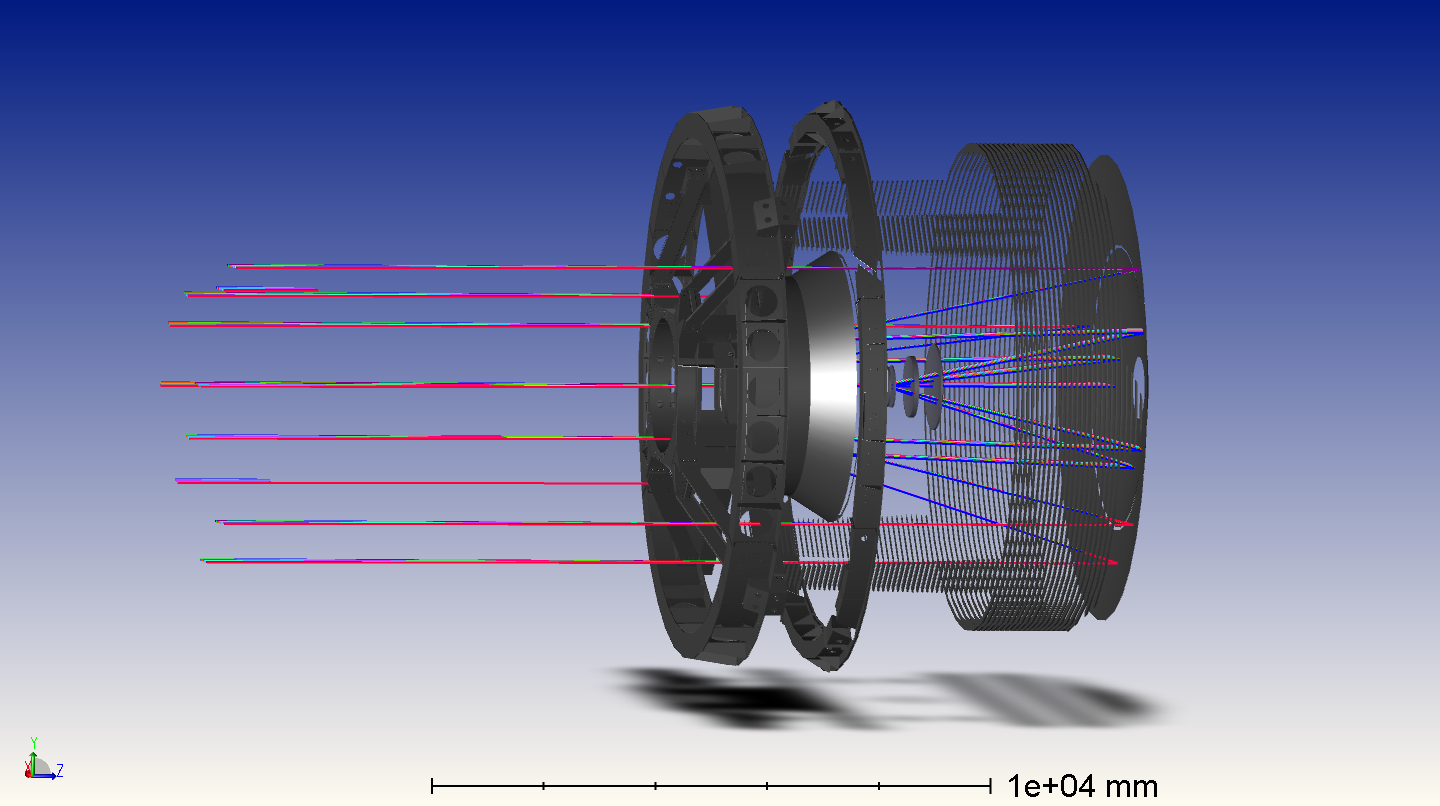
\includegraphics[height=7.5cm]{Rubin_effective_area_baffles}
\end{tabular}
\end{center}
\caption 
{ \label{baffles} View of the Rubin telescope's 3D non-sequential ray tracing model and its main mechanical components relevant to the study.}
\end{figure} 

The pupil obstruction geometry by the TEA is shown in Fig.  \ref{off_obs}.

\begin{figure}
\begin{center}
\begin{tabular}{c}
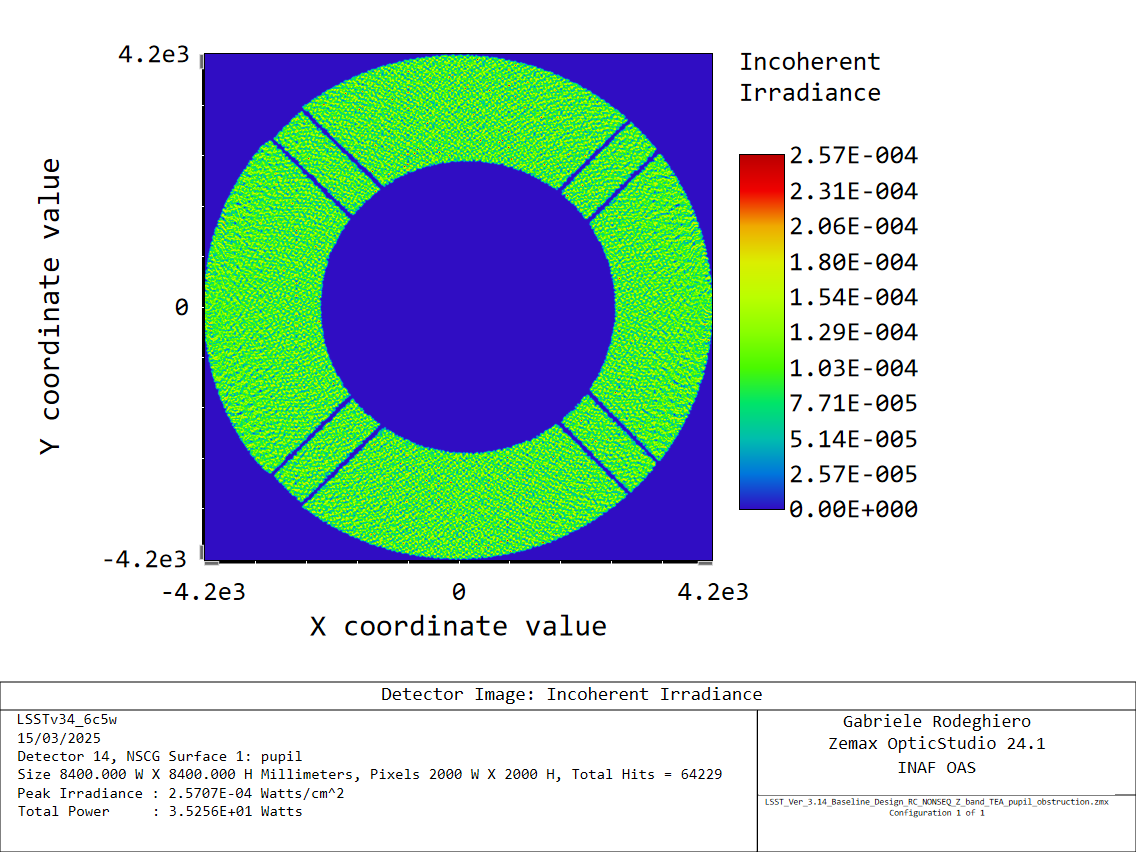
\includegraphics[height=7.5cm]{Off-axis-obscuration}
\end{tabular}
\end{center}
\caption 
{ \label{off_obs} Geometry of the pupil obstruction for the LSSTCam outermost field (1.75$^\circ$) derived from the ray tracing simulations. The TEA obstruction factor increases for a geometric projection effect for off-axis positions.}
\end{figure} 



The reflectance data from the primary and tertiary mirror (M1M3) and secondary mirror (M2) have been measured and monitored over time by \cite{M1M2M3_Vucina}. The Rubin mirrors are coated with protected Silver, and their measured reflectance profile is reported in Fig. \ref{m1m2m3}.

\begin{figure}
\begin{center}
\begin{tabular}{c}
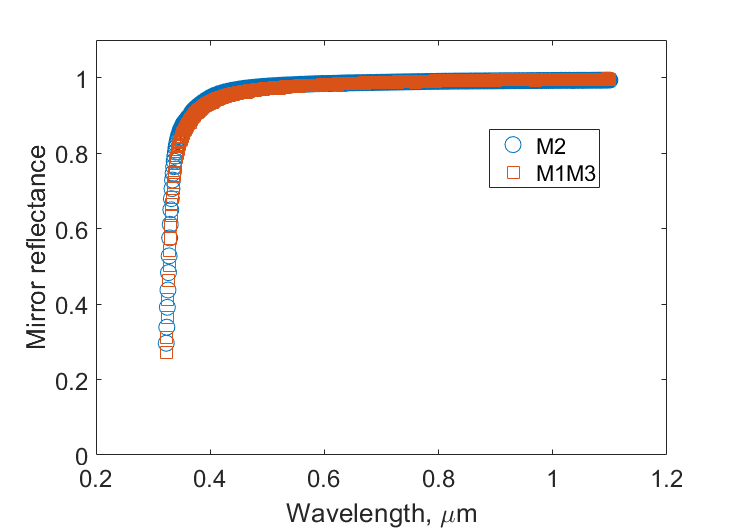
\includegraphics[height=8cm]{M1M2M3_reflectance}
\end{tabular}
\end{center}
\caption 
{ \label{m1m2m3} Measured reflectance (normalized value) for the M1M3 and M2 mirrors used for the telescope effective area calculations.}
\end{figure} 


The LSSTCam throughput (Fig. \ref{L1L2L3QE}) has been measured by \cite{LSSTCam_Andy} through the three LSSTCam lenses (L1, L2, L3), including the detectors QE. A separate set of transmission measurements for the six filters is reported in the same repository by \cite{LSSTCam_Andy}. The bandpass profiles of the filters and their variation with the photon angles of incidence are reported in Fig. \ref{filters} and \ref{g_filter}, respectively.
The source data are organized to filter different transmission curves (u,g,r,i,z,y) and the two types of detectors (ITL \& e2v). The LSSTCam focal plane has 13x9 $\rightarrow$ 117 e2v and 8x9 $\rightarrow$  72 ITL sensors, which translates into a 61.9\% weighting of the e2v and 38.1\% of the ITL QE curve. The average QE of the LSSTCam focal plane is represented by adding the detector's QE in the proportion between e2v and ITL detectors.


\begin{figure}
\begin{center}
\begin{tabular}{c}
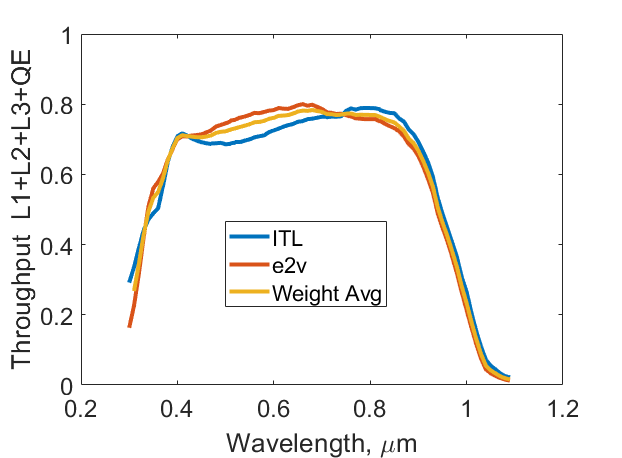
\includegraphics[height=7cm]{LSSTCam_lens_QE}
\end{tabular}
\end{center}
\caption 
{ \label{L1L2L3QE} Measured throughput (normalized value) of the optical assembly L1+L2+L3+Detector QE. The LSSTCam focal plane has 117 e2v detectors and 72 ITL sensors; the yellow curve is the weighted average over the whole LSSTCam focal plane for 61.9\% of the e2v and 38.1\% of the ITL QE.}
\end{figure} 


\begin{figure}
\begin{center}
\begin{tabular}{c}
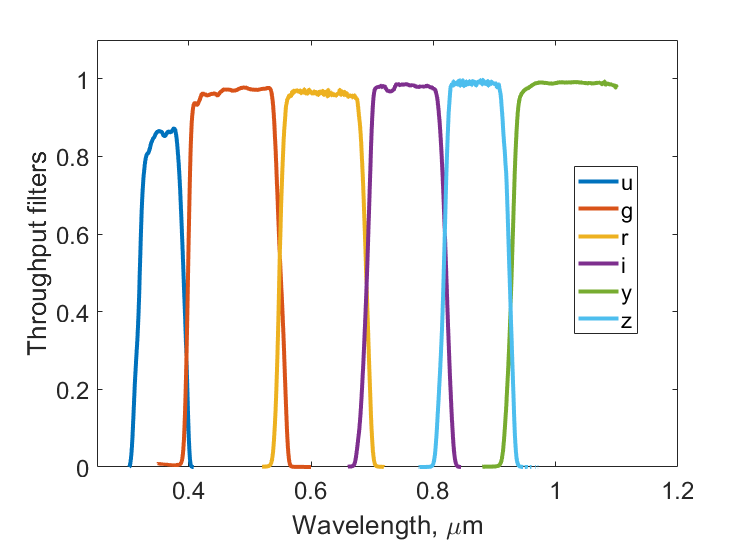
\includegraphics[height=7cm]{Filters_transmission_rubin}
\end{tabular}
\end{center}
\caption 
{ \label{filters} Measured transmittance (normalized value) and bandpass profile for the six LSSTCam optical filters.}
\end{figure} 


\begin{figure}
\begin{center}
\begin{tabular}{c}
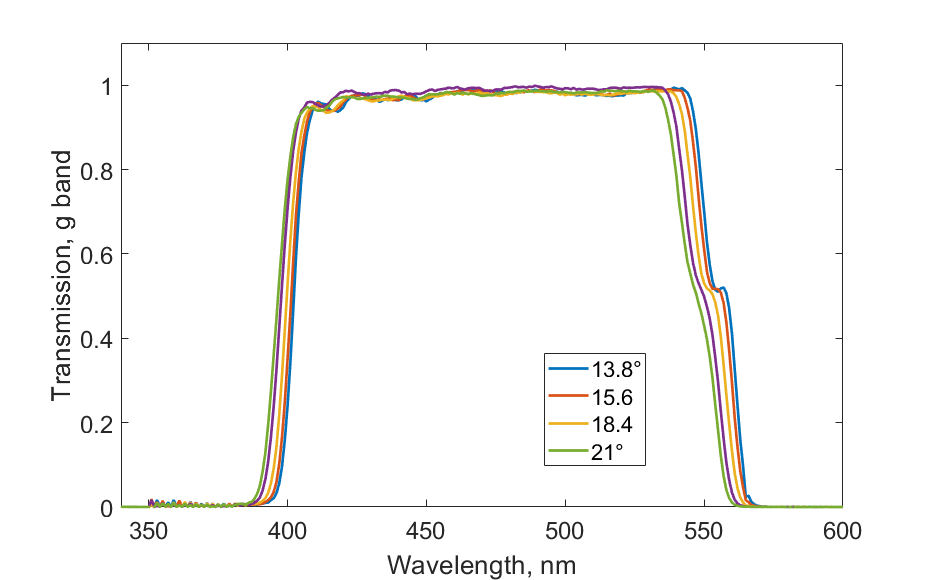
\includegraphics[height=8cm]{g_band_filter_AoI_Rubin}
\end{tabular}
\end{center}
\caption 
{ \label{g_filter} Example of filter bandpass transmittance for different photon angles of incidence.}
\end{figure} 


\clearpage

\section{Rubin effective area calculations} 

The estimation of the Rubin effective area for different positions within the Field of View (FoV) of the LSSTCam and for the six optical filters is reported in Fig. \ref{eff}. The effective area is expressed in $m^2$ and is derived assuming an input flux at the telescope entrance pupil F = 54.89 W; the flux corresponds to the area of the telescope entrance pupil $A_{EnPup}$ = $\pi\times r_{M1}^2$. The decrease of the effective area along the FoV is due to the increase of the TEA obstruction projection for the off-axis fields (Fig. \ref{off_obs}). The low effective area in the $u$ band is due to the lower mirror reflectance and detector QE.


\begin{figure}
\begin{center}
\begin{tabular}{c}
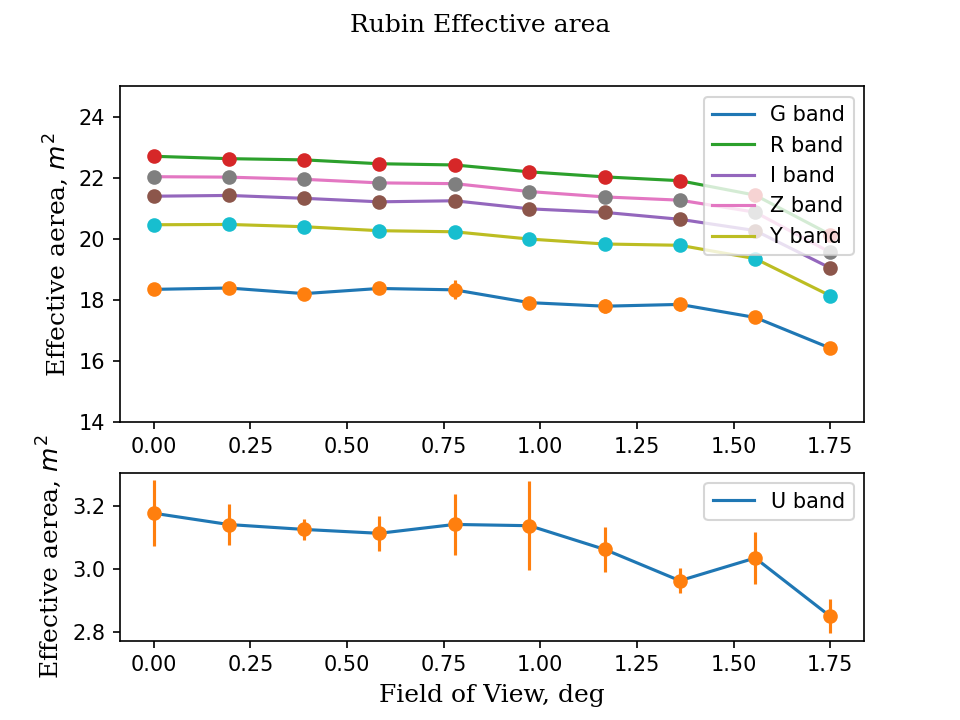
\includegraphics[height=10cm]{Rubin_effective_area_TEA_cad}
\end{tabular}
\end{center}
\caption 
{ \label{eff} Estimated Rubin effective area from non-sequential ray tracing simulations within the six optical filters and for different off-axis fields.}
\end{figure} 



The effective area values for different filters and field positions in the FoV are tabulated in Table \ref{eff_table} and available in the \cite{sitcom} folder. The values are determined as the average effective area over five MonteCarlo simulations with the RMS as statistical uncertainty.  


\begin{table*}
\begin{center}
\begin{tabular}{p{1.4cm}*{7}{c}} \hline

Off-axis field & $REA_u$ & $REA_g$ & $REA_r$ & $REA_i$ & $REA_z$ & $REA_y$\\
\hline
0$^\circ$ & 9.20 $\pm$ 0.15 & 20.79 $\pm$ 0.05 & 23.16 $\pm$ 0.03 & 23.66 $\pm$  0.01 & 22.14 $\pm$  0.03 & 9.74 $\pm$ 0.06 \\
0.19$^\circ$ & 9.25 $\pm$  0.09 & 20.70 $\pm$  0.03 & 23.07 $\pm$  0.02 & 23.60 $\pm$ 0.03 & 22.06 $\pm$ 0.06 & 9.72  $\pm$ 0.12 \\
0.39$^\circ$ & 9.28 $\pm$  0.12 & 20.72 $\pm$  0.05 & 23.05 $\pm$  0.05 & 23.56 $\pm$  0.02 & 22.05 $\pm$ 0.04 & 9.83 $\pm$  0.03 \\
0.58$^\circ$ & 9.23 $\pm$ 0.14 & 20.59 $\pm$  0.04 & 22.90 $\pm$  0.03 & 23.40 $\pm$ 0.02 & 21.90 $\pm$ 0.09 & 9.76  $\pm$  0.16 \\
0.78$^\circ$ & 9.29 $\pm$  0.13 & 20.52 $\pm$  0.04 &22.84  $\pm$  0.02 & 23.35 $\pm$  0.02 & 21.90 $\pm$ 0.08 & 9.59 $\pm$  0.07 \\
0.97$^\circ$ & 9.00 $\pm$  0.09 & 20.36 $\pm$  0.05 & 22.69 $\pm$  0.02 & 23.15 $\pm$  0.02 & 21.69 $\pm$ 0.02 & 9.66  $\pm$  0.12 \\
1.17$^\circ$ & 9.07 $\pm$  0.11 & 20.27 $\pm$  0.05 & 22.56 $\pm$  0.03 & 23.05 $\pm$  0.02 & 21.58 $\pm$ 0.03 & 9.55  $\pm$  0.10\\
1.36$^\circ$ & 8.94 $\pm$  0.06 & 20.06 $\pm$  0.04 & 22.33 $\pm$  0.03 & 22.82 $\pm$  0.02 & 21.37 $\pm$ 0.10 & 9.47  $\pm$  0.15\\
1.55$^\circ$ & 8.86 $\pm$  0.09 & 19.64 $\pm$  0.05 & 21.85 $\pm$  0.01 & 22.34 $\pm$  0.01 & 20.92 $\pm$ 0.03 & 9.2  $\pm$ 0.04\\
1.75$^\circ$ & 8.41  $\pm$ 0.11 & 18.64 $\pm$  0.02 & 20.73 $\pm$  0.03 & 21.14 $\pm$  0.02 & 19.79 $\pm$  0.03 & 8.76  $\pm$ 0.07\\


\hline
\end{tabular}
\caption{Rubin estimated effective area $REA$ through the six filters and for different off-axis fields.\label{eff_table} Units are $m^2$.}
 \end{center}
 \end{table*}



\clearpage


\appendix
% Include all the relevant bib files.
% https://lsst-texmf.lsst.io/lsstdoc.html#bibliographies
\section{References} \label{sec:bib}
\renewcommand{\refname}{} % Suppress default Bibliography section
\bibliography{local,lsst,lsst-dm,refs_ads,refs,books}

% Make sure lsst-texmf/bin/generateAcronyms.py is in your path
\section{Acronyms} \label{sec:acronyms}
\addtocounter{table}{-1}
\begin{longtable}{p{0.145\textwidth}p{0.8\textwidth}}\hline
\textbf{Acronym} & \textbf{Description}  \\\hline

3D & Three-dimensional \\\hline
FoV & Field of View (also denoted FOV) \\\hline
ITL & Imaging Technology Laboratory (UA) \\\hline
L1 & Lens 1 \\\hline
L2 & Lens 2 \\\hline
L3 & Lens 3 \\\hline
M1 & primary mirror \\\hline
M1M3 & Primary Mirror Tertiary Mirror \\\hline
M2 & Secondary Mirror \\\hline
OSS & Observatory System Specifications; LSE-30 \\\hline
QE & quantum efficiency \\\hline
SE & System Engineering \\\hline
SST & Subsystem Science Team \\\hline
TEA & Top End Assembly \\\hline
TMA & Telescope Mount Assembly \\\hline
\end{longtable}

% If you want glossary uncomment below -- comment out the two lines above
%\printglossaries






\end{document}
